\documentclass[twoside]{book}

% Packages required by doxygen
\usepackage{fixltx2e}
\usepackage{calc}
\usepackage{doxygen}
\usepackage[export]{adjustbox} % also loads graphicx
\usepackage{graphicx}
\usepackage[utf8]{inputenc}
\usepackage{makeidx}
\usepackage{multicol}
\usepackage{multirow}
\PassOptionsToPackage{warn}{textcomp}
\usepackage{textcomp}
\usepackage[nointegrals]{wasysym}
\usepackage[table]{xcolor}

% Font selection
\usepackage[T1]{fontenc}
\usepackage[scaled=.90]{helvet}
\usepackage{courier}
\usepackage{amssymb}
\usepackage{sectsty}
\renewcommand{\familydefault}{\sfdefault}
\allsectionsfont{%
  \fontseries{bc}\selectfont%
  \color{darkgray}%
}
\renewcommand{\DoxyLabelFont}{%
  \fontseries{bc}\selectfont%
  \color{darkgray}%
}
\newcommand{\+}{\discretionary{\mbox{\scriptsize$\hookleftarrow$}}{}{}}

% Page & text layout
\usepackage{geometry}
\geometry{%
  a4paper,%
  top=2.5cm,%
  bottom=2.5cm,%
  left=2.5cm,%
  right=2.5cm%
}
\tolerance=750
\hfuzz=15pt
\hbadness=750
\setlength{\emergencystretch}{15pt}
\setlength{\parindent}{0cm}
\setlength{\parskip}{0.2cm}
\makeatletter
\renewcommand{\paragraph}{%
  \@startsection{paragraph}{4}{0ex}{-1.0ex}{1.0ex}{%
    \normalfont\normalsize\bfseries\SS@parafont%
  }%
}
\renewcommand{\subparagraph}{%
  \@startsection{subparagraph}{5}{0ex}{-1.0ex}{1.0ex}{%
    \normalfont\normalsize\bfseries\SS@subparafont%
  }%
}
\makeatother

% Headers & footers
\usepackage{fancyhdr}
\pagestyle{fancyplain}
\fancyhead[LE]{\fancyplain{}{\bfseries\thepage}}
\fancyhead[CE]{\fancyplain{}{}}
\fancyhead[RE]{\fancyplain{}{\bfseries\leftmark}}
\fancyhead[LO]{\fancyplain{}{\bfseries\rightmark}}
\fancyhead[CO]{\fancyplain{}{}}
\fancyhead[RO]{\fancyplain{}{\bfseries\thepage}}
\fancyfoot[LE]{\fancyplain{}{}}
\fancyfoot[CE]{\fancyplain{}{}}
\fancyfoot[RE]{\fancyplain{}{\bfseries\scriptsize Generated on Sun Mar 15 2015 08\+:56\+:09 for A\+I Robot with mbed by Doxygen }}
\fancyfoot[LO]{\fancyplain{}{\bfseries\scriptsize Generated on Sun Mar 15 2015 08\+:56\+:09 for A\+I Robot with mbed by Doxygen }}
\fancyfoot[CO]{\fancyplain{}{}}
\fancyfoot[RO]{\fancyplain{}{}}
\renewcommand{\footrulewidth}{0.4pt}
\renewcommand{\chaptermark}[1]{%
  \markboth{#1}{}%
}
\renewcommand{\sectionmark}[1]{%
  \markright{\thesection\ #1}%
}

% Indices & bibliography
\usepackage{natbib}
\usepackage[titles]{tocloft}
\setcounter{tocdepth}{3}
\setcounter{secnumdepth}{5}
\makeindex

% Hyperlinks (required, but should be loaded last)
\usepackage{ifpdf}
\ifpdf
  \usepackage[pdftex,pagebackref=true]{hyperref}
\else
  \usepackage[ps2pdf,pagebackref=true]{hyperref}
\fi
\hypersetup{%
  colorlinks=true,%
  linkcolor=blue,%
  citecolor=blue,%
  unicode%
}

% Custom commands
\newcommand{\clearemptydoublepage}{%
  \newpage{\pagestyle{empty}\cleardoublepage}%
}


%===== C O N T E N T S =====

\begin{document}

% Titlepage & ToC
\hypersetup{pageanchor=false,
             bookmarks=true,
             bookmarksnumbered=true,
             pdfencoding=unicode
            }
\pagenumbering{roman}
\begin{titlepage}
\vspace*{7cm}
\begin{center}%
{\Large A\+I Robot with mbed }\\
\vspace*{1cm}
{\large Generated by Doxygen 1.8.9.1}\\
\vspace*{0.5cm}
{\small Sun Mar 15 2015 08:56:09}\\
\end{center}
\end{titlepage}
\clearemptydoublepage
\tableofcontents
\clearemptydoublepage
\pagenumbering{arabic}
\hypersetup{pageanchor=true}

%--- Begin generated contents ---
\chapter{Class Index}
\section{Class List}
Here are the classes, structs, unions and interfaces with brief descriptions\+:\begin{DoxyCompactList}
\item\contentsline{section}{\hyperlink{class_device_address}{Device\+Address} }{\pageref{class_device_address}}{}
\item\contentsline{section}{\hyperlink{class_x_bee_data_frame_builder}{X\+Bee\+Data\+Frame\+Builder} }{\pageref{class_x_bee_data_frame_builder}}{}
\end{DoxyCompactList}

\chapter{File Index}
\section{File List}
Here is a list of all documented files with brief descriptions\+:\begin{DoxyCompactList}
\item\contentsline{section}{Wireless\+Communication/\hyperlink{_device_address_8h}{Device\+Address.\+h} \\*64byte X\+Bee address }{\pageref{_device_address_8h}}{}
\item\contentsline{section}{Wireless\+Communication/{\bfseries X\+Bee\+Data\+Frame\+Builder.\+h} }{\pageref{_x_bee_data_frame_builder_8h}}{}
\end{DoxyCompactList}

\chapter{Class Documentation}
\hypertarget{class_a_p_i_frame}{}\section{A\+P\+I\+Frame Class Reference}
\label{class_a_p_i_frame}\index{A\+P\+I\+Frame@{A\+P\+I\+Frame}}
\subsection*{Public Member Functions}
\begin{DoxyCompactItemize}
\item 
\hypertarget{class_a_p_i_frame_a49e61a04eb3a88c219e123dbc5776bf3}{}{\bfseries A\+P\+I\+Frame} (uint8\+\_\+t $\ast$frame\+Data, int \&Length)\label{class_a_p_i_frame_a49e61a04eb3a88c219e123dbc5776bf3}

\item 
\hypertarget{class_a_p_i_frame_a99d27f3be177320fc342157837a1a980}{}uint8\+\_\+t {\bfseries Get\+Frame\+Data\+Length} () const \label{class_a_p_i_frame_a99d27f3be177320fc342157837a1a980}

\item 
\hypertarget{class_a_p_i_frame_a2af55b4ac6145666fe9e56e5c4fd6184}{}const uint8\+\_\+t $\ast$ {\bfseries Get\+Frame\+Data} () const \label{class_a_p_i_frame_a2af55b4ac6145666fe9e56e5c4fd6184}

\end{DoxyCompactItemize}
\subsection*{Protected Attributes}
\begin{DoxyCompactItemize}
\item 
\hypertarget{class_a_p_i_frame_a6811a17e535f4601c3acbcde0f36c48a}{}int {\bfseries Frame\+Data\+Length}\label{class_a_p_i_frame_a6811a17e535f4601c3acbcde0f36c48a}

\item 
\hypertarget{class_a_p_i_frame_aa447c31d400fd8d96cf89ee2a8e3dbc1}{}std\+::vector$<$ uint8\+\_\+t $>$ {\bfseries Frame\+Data}\label{class_a_p_i_frame_aa447c31d400fd8d96cf89ee2a8e3dbc1}

\end{DoxyCompactItemize}


The documentation for this class was generated from the following file\+:\begin{DoxyCompactItemize}
\item 
Wireless\+Communication/\hyperlink{_a_p_i_frame_8h}{A\+P\+I\+Frame.\+h}\end{DoxyCompactItemize}

\hypertarget{class_device_address}{}\section{Device\+Address Class Reference}
\label{class_device_address}\index{Device\+Address@{Device\+Address}}
\subsection*{Public Member Functions}
\begin{DoxyCompactItemize}
\item 
\hypertarget{class_device_address_a47393b85f2d963195e13732bf1b92ebe}{}{\bfseries Device\+Address} (const uint8\+\_\+t $\ast$msb\+\_\+lsb\+\_\+net)\label{class_device_address_a47393b85f2d963195e13732bf1b92ebe}

\item 
\hypertarget{class_device_address_a23700d852405505711181eff85190f7a}{}{\bfseries Device\+Address} (const uint8\+\_\+t $\ast$msb\+\_\+lsb, const uint8\+\_\+t $\ast$net)\label{class_device_address_a23700d852405505711181eff85190f7a}

\item 
\hypertarget{class_device_address_a401795eb7df3cbe4f6e6b70adf9b0f13}{}{\bfseries Device\+Address} (uint32\+\_\+t msb, uint32\+\_\+t lsb, uint16\+\_\+t net)\label{class_device_address_a401795eb7df3cbe4f6e6b70adf9b0f13}

\item 
\hypertarget{class_device_address_a57bc48e59d6d8bb17b74d8b7c0f19b0e}{}uint32\+\_\+t {\bfseries Get\+M\+S\+B} () const \label{class_device_address_a57bc48e59d6d8bb17b74d8b7c0f19b0e}

\item 
\hypertarget{class_device_address_a452ba13a7c3d4c79af1689eb4b81d7ab}{}uint32\+\_\+t {\bfseries Get\+L\+S\+B} () const \label{class_device_address_a452ba13a7c3d4c79af1689eb4b81d7ab}

\item 
\hypertarget{class_device_address_a354bd15b0235c27cc69a04a04fda5938}{}uint16\+\_\+t {\bfseries Get\+N\+E\+T} () const \label{class_device_address_a354bd15b0235c27cc69a04a04fda5938}

\item 
\hypertarget{class_device_address_a249dd92571ea9001ff02063229bc5283}{}const uint8\+\_\+t $\ast$ {\bfseries Get\+Value} () const \label{class_device_address_a249dd92571ea9001ff02063229bc5283}

\end{DoxyCompactItemize}
\subsection*{Protected Attributes}
\begin{DoxyCompactItemize}
\item 
\hypertarget{class_device_address_a52af8f243ce02cd6aa3798ff8c91bbce}{}std\+::vector$<$ uint8\+\_\+t $>$ {\bfseries value}\label{class_device_address_a52af8f243ce02cd6aa3798ff8c91bbce}

\end{DoxyCompactItemize}
\subsection*{Friends}
\begin{DoxyCompactItemize}
\item 
\hypertarget{class_device_address_ad12612d4bc462ca3e4f3fc9b5891cc4d}{}bool {\bfseries operator==} (const \hyperlink{class_device_address}{Device\+Address} \&a, const \hyperlink{class_device_address}{Device\+Address} \&b)\label{class_device_address_ad12612d4bc462ca3e4f3fc9b5891cc4d}

\item 
\hypertarget{class_device_address_a6baeb447978c5a7bd562573559a68357}{}bool {\bfseries operator!=} (const \hyperlink{class_device_address}{Device\+Address} \&a, const \hyperlink{class_device_address}{Device\+Address} \&b)\label{class_device_address_a6baeb447978c5a7bd562573559a68357}

\end{DoxyCompactItemize}


The documentation for this class was generated from the following file\+:\begin{DoxyCompactItemize}
\item 
Wireless\+Communication/\hyperlink{_device_address_8h}{Device\+Address.\+h}\end{DoxyCompactItemize}

\hypertarget{class_x_bee_a_p_i_frame_builder}{}\section{X\+Bee\+A\+P\+I\+Frame\+Builder Class Reference}
\label{class_x_bee_a_p_i_frame_builder}\index{X\+Bee\+A\+P\+I\+Frame\+Builder@{X\+Bee\+A\+P\+I\+Frame\+Builder}}
\subsection*{Public Member Functions}
\begin{DoxyCompactItemize}
\item 
\hypertarget{class_x_bee_a_p_i_frame_builder_a7cbca7791e2fe53d237648d38010c147}{}{\bfseries X\+Bee\+A\+P\+I\+Frame\+Builder} (uint8\+\_\+t Frame\+I\+D, const )\label{class_x_bee_a_p_i_frame_builder_a7cbca7791e2fe53d237648d38010c147}

\item 
\hypertarget{class_x_bee_a_p_i_frame_builder_af0bcd1cf3efac52cef4775ccd2d05144}{}{\bfseries build} ()\label{class_x_bee_a_p_i_frame_builder_af0bcd1cf3efac52cef4775ccd2d05144}

\end{DoxyCompactItemize}


The documentation for this class was generated from the following file\+:\begin{DoxyCompactItemize}
\item 
Wireless\+Communication/\hyperlink{_x_bee_a_p_i_frame_builder_8h}{X\+Bee\+A\+P\+I\+Frame\+Builder.\+h}\end{DoxyCompactItemize}

\chapter{File Documentation}
\hypertarget{_a_p_i_frame_8h}{}\section{Wireless\+Communication/\+A\+P\+I\+Frame.h File Reference}
\label{_a_p_i_frame_8h}\index{Wireless\+Communication/\+A\+P\+I\+Frame.\+h@{Wireless\+Communication/\+A\+P\+I\+Frame.\+h}}


A\+P\+I frame value object.  


{\ttfamily \#include $<$vector$>$}\\*
{\ttfamily \#include \char`\"{}stdint.\+h\char`\"{}}\\*
Include dependency graph for A\+P\+I\+Frame.\+h\+:
\nopagebreak
\begin{figure}[H]
\begin{center}
\leavevmode
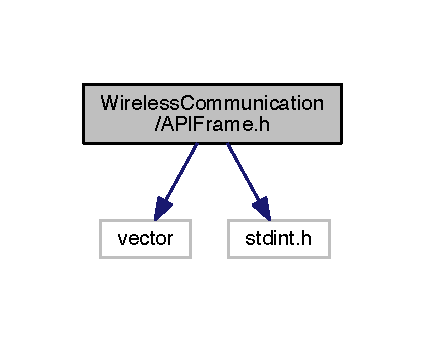
\includegraphics[width=204pt]{_a_p_i_frame_8h__incl}
\end{center}
\end{figure}
\subsection*{Classes}
\begin{DoxyCompactItemize}
\item 
class \hyperlink{class_a_p_i_frame}{A\+P\+I\+Frame}
\end{DoxyCompactItemize}


\subsection{Detailed Description}
A\+P\+I frame value object. 

\begin{DoxyAuthor}{Author}
Soichi 
\end{DoxyAuthor}
\begin{DoxyDate}{Date}
2015-\/03-\/15 08\+:55\+:24 Sunday reference\+: \href{https://developer.mbed.org/users/yangcq88517/code/SmartLabXBeeAPI/file/e863071f1c9e/Type/APIFrame.h}{\tt https\+://developer.\+mbed.\+org/users/yangcq88517/code/\+Smart\+Lab\+X\+Bee\+A\+P\+I/file/e863071f1c9e/\+Type/\+A\+P\+I\+Frame.\+h} 
\end{DoxyDate}

\hypertarget{_device_address_8h}{}\section{Wireless\+Communication/\+Device\+Address.h File Reference}
\label{_device_address_8h}\index{Wireless\+Communication/\+Device\+Address.\+h@{Wireless\+Communication/\+Device\+Address.\+h}}


64byte X\+Bee address  


{\ttfamily \#include $<$vector$>$}\\*
{\ttfamily \#include \char`\"{}stdint.\+h\char`\"{}}\\*
Include dependency graph for Device\+Address.\+h\+:\nopagebreak
\begin{figure}[H]
\begin{center}
\leavevmode
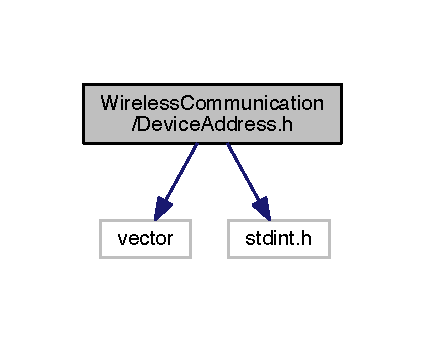
\includegraphics[width=204pt]{_device_address_8h__incl}
\end{center}
\end{figure}
\subsection*{Classes}
\begin{DoxyCompactItemize}
\item 
class \hyperlink{class_device_address}{Device\+Address}
\end{DoxyCompactItemize}


\subsection{Detailed Description}
64byte X\+Bee address 

X\+Bee device address reference\+: \href{https://developer.mbed.org/users/yangcq88517/code/SmartLabXBeeAPI/file/e863071f1c9e/Type/DeviceAddress.h}{\tt https\+://developer.\+mbed.\+org/users/yangcq88517/code/\+Smart\+Lab\+X\+Bee\+A\+P\+I/file/e863071f1c9e/\+Type/\+Device\+Address.\+h}

\begin{DoxyAuthor}{Author}
Soichi 
\end{DoxyAuthor}
\begin{DoxyDate}{Date}
2015-\/03-\/15 08\+:06\+:39 Sunday 
\end{DoxyDate}

\hypertarget{_x_bee_a_p_i_frame_builder_8h}{}\section{Wireless\+Communication/\+X\+Bee\+A\+P\+I\+Frame\+Builder.h File Reference}
\label{_x_bee_a_p_i_frame_builder_8h}\index{Wireless\+Communication/\+X\+Bee\+A\+P\+I\+Frame\+Builder.\+h@{Wireless\+Communication/\+X\+Bee\+A\+P\+I\+Frame\+Builder.\+h}}


build X\+Bee A\+P\+I frame  


{\ttfamily \#include $<$string$>$}\\*
Include dependency graph for X\+Bee\+A\+P\+I\+Frame\+Builder.\+h\+:
\nopagebreak
\begin{figure}[H]
\begin{center}
\leavevmode
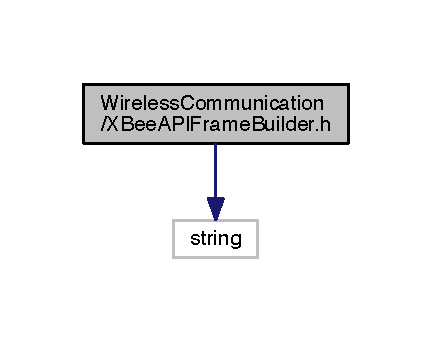
\includegraphics[width=207pt]{_x_bee_a_p_i_frame_builder_8h__incl}
\end{center}
\end{figure}
\subsection*{Classes}
\begin{DoxyCompactItemize}
\item 
class \hyperlink{class_x_bee_a_p_i_frame_builder}{X\+Bee\+A\+P\+I\+Frame\+Builder}
\end{DoxyCompactItemize}


\subsection{Detailed Description}
build X\+Bee A\+P\+I frame 

\begin{DoxyAuthor}{Author}
Soichi 
\end{DoxyAuthor}
\begin{DoxyDate}{Date}
2015-\/03-\/15 08\+:28\+:35 Sunday 
\end{DoxyDate}

%--- End generated contents ---

% Index
\backmatter
\newpage
\phantomsection
\clearemptydoublepage
\addcontentsline{toc}{chapter}{Index}
\printindex

\end{document}
